\begin{center}
    \Huge{\textbf{\underline{Chapter 1: Python Basics}}}
\end{center}

\setcounter{section}{0}

\vspace{0.25cm}

\section{Introduction}
\begin{prettyBox}{Introduction}{myblue}
Python is a dynamically typed programming language, meaning that we don't  
have to specify the type of function parameters or variables, the interpreter  
takes care of it.
\end{prettyBox}

\vspace{0.45cm}

\section{Types}
\begin{prettyBox}{Types}{myblue}
Like any programming language, Python offers two types of data types:
\begin{itemize}
    \item \textbf{Primitive}: Stores simple, single values that are immutable.
    \item \textbf{Non-Primitive}: Stores collections of complex values that are usually mutable, with some exceptions.
\end{itemize}
\end{prettyBox}

\vspace{0.25cm}
\subsection{Primitive Types}
\begin{prettyBox}{Primitive Types}{myblue}
\begin{itemize}
    \item \textbf{int}: Integer numerical value.
    \item \textbf{float}: Decimal numerical value.
    \item \textbf{string}: Sequence of characters.
    \item \textbf{boolean}: Represents \texttt{True} or \texttt{False}.
\end{itemize}
\end{prettyBox}

\vspace{0.25cm}
\subsection{Non-Primitive Types}
\begin{prettyBox}{Non-Primitive Types}{myblue}
\begin{itemize}
    \item \textbf{list}: Stores an ordered collection of values.
    \item \textbf{tuple}: Similar to a list but we can't change their value directly only overide the whole
        tuple with a new one.
    \item \textbf{set}: Stores a collection of unordered, unique values.
    \item \textbf{dictionary}: A mapping data structure where each element is a key-value pair.
\end{itemize}
\end{prettyBox}



\textbf{\underline{Primitive Example}}\\[0.1cm]
\lstinputlisting[style=pythonstyle]{Chapters/Code/Basics/Types/prim.py}

\vspace{0.25cm}
\begin{center}
    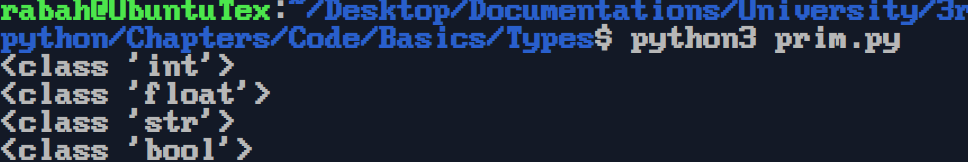
\includegraphics[width = 0.9\textwidth]{Chapters/ScreenShot/Basics/Types/primOutput.png}
\end{center}

\vspace{1cm}

\textbf{\underline{Non Primitive Example}}\\[0.1cm]
\lstinputlisting[style=pythonstyle]{Chapters/Code/Basics/Types/NonPrim.py}

\vspace{0.25cm}
\begin{center}
    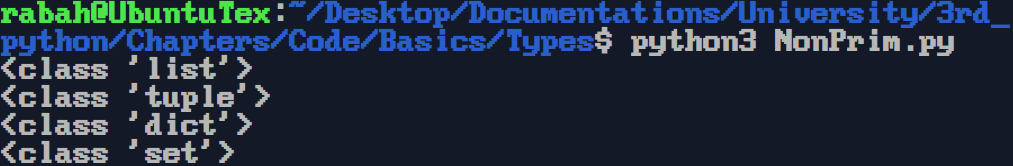
\includegraphics[width = 0.9\textwidth]{Chapters/ScreenShot/Basics/Types/NonPrimOutput.png}
\end{center}

\vspace{0.5cm}


\section{Comments}
\begin{prettyBox}{Comments}{myblue}
\begin{itemize}
    \item Single Line Comment : they start with \#
    \item Multi-Line Block Comment : wrapped between single or double quote : \texttt{'''} , \texttt{"""}
\end{itemize}
\end{prettyBox}

\vspace{0.35cm}
\textbf{\underline{Example}}\\[0.1cm]
\lstinputlisting[style=pythonstyle]{Chapters/Code/Basics/Comments/com.py}

\vspace{0.25cm}
\begin{center}
    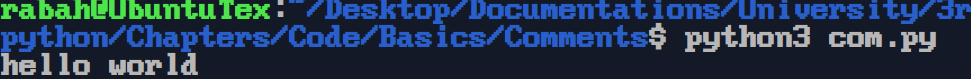
\includegraphics[width = 0.9\textwidth]{Chapters/ScreenShot/Basics/Comments/comOutput.png}
\end{center}

\vspace{1cm}
\section{Input/Output}
\begin{prettyBox}{IO}{myblue}
\begin{itemize}
    \item \texttt{print} : we use the print function to display text , 
        there are many string formatting we will see them in next section , the default formating
        is text between qout and we seprate variable with comma , and it automatically add space
    \item \texttt{input} : has message inside ,by default input takes in string variable.we can type
        cast it , we can input many var at once with split() , we use map when inputing many var + 
        typecasting
\end{itemize}
\end{prettyBox}

\vspace{0.5cm}
\textbf{\underline{Syntax}}\\[0.1cm]
\lstinputlisting[style=pythonstyle]{Chapters/Code/Basics/IO/syn.py}

\newpage
\textbf{\underline{Example}}\\[0.1cm]
\lstinputlisting[style=pythonstyle]{Chapters/Code/Basics/IO/io.py}


\vspace{0.25cm}
\begin{center}
    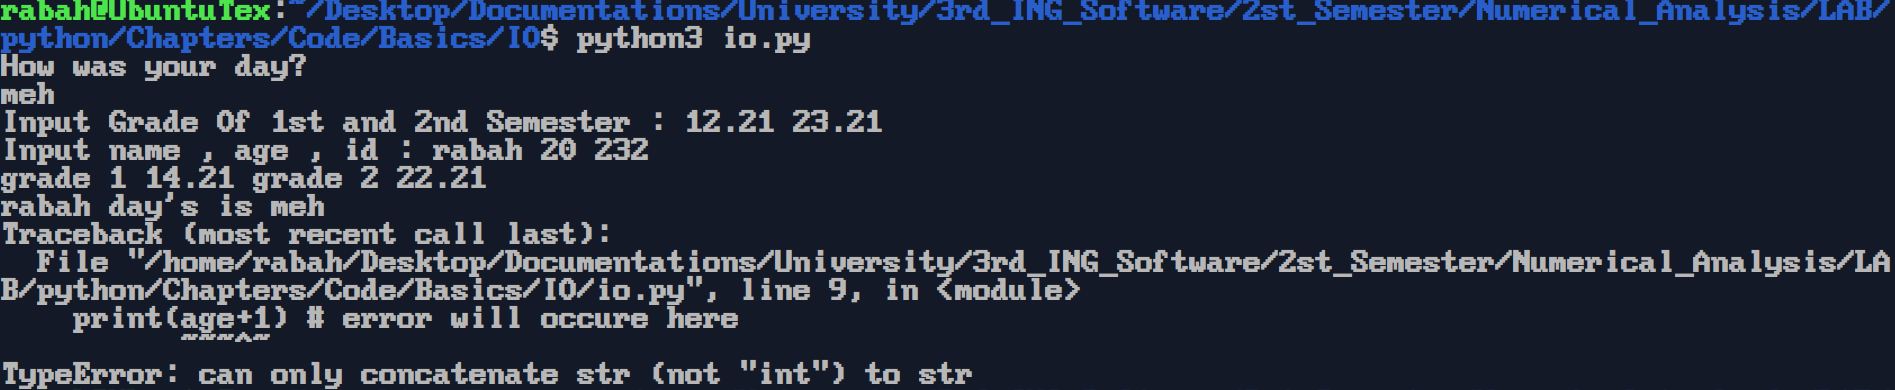
\includegraphics[width = 0.9\textwidth]{Chapters/ScreenShot/Basics/IO/ioOutput.png}
\end{center}

\vspace{1cm}
\section{String Formatting}

\begin{prettyBox}{Formatting}{myblue}
\begin{itemize}
    \item Default : Uses \texttt{print()} with values separated by commas, automatically adding spaces.
    \item f-string : Uses \texttt{f"\{var\}"}, treats \texttt{\textbackslash} as an escape character, and what's between \texttt{\{\}} is evaluated as a variable , Use \texttt{\{\{\}\}} for literal curly braces.
    \item raw-string : Uses \texttt{r"string"} to treat backslashes \texttt{\textbackslash} as literal characters.
    \item f+raw-string : Uses \texttt{fr"string"}, supports \texttt{\{var\}} formatting of f-string while treating \texttt{\textbackslash} as a literal character.
\item \% formatting : Uses \texttt{"format \% value"}, similar to C-style formatting.
    \item .format : Uses \texttt{"\{\} \{\}".format(val1, val2)} to insert values into placeholders. Placeholders can be empty, indexed, or labeled.
\end{itemize}
\end{prettyBox}

\vspace{0.5cm}

\newpage
\textbf{\underline{Example}}\\[0.1cm]
\lstinputlisting[style=pythonstyle]{Chapters/Code/Basics/Format/form.py}


\vspace{0.25cm}
\begin{center}
    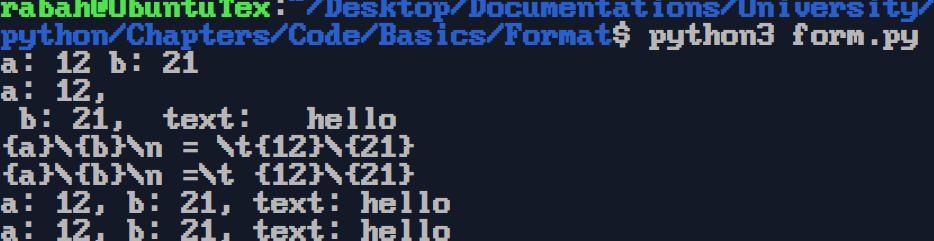
\includegraphics[width = 0.9\textwidth]{Chapters/ScreenShot/Basics/Format/formatOutput.png}
\end{center}

\vspace{1cm}

\section{Importing Modules}

\begin{prettyBox}{Import}{myblue}
A module in Python is simply a file containing Python code with classes , functions and variables that we can include and use in our own programs. There are two main ways to import modules:
\begin{itemize}
    \item \textbf{Importing the entire module}: This loads all the module’s functions, classes, and variables , to access them we need to
        write the modulename followed by a point
    \item \textbf{Importing specific parts of a module}: Instead of loading everything, we can import only specific functions, classes, or variables, which
        we call directly by their name.
\end{itemize}
\end{prettyBox}

\vspace{0.5cm}

\begin{prettyBox}{Note}{red}
\begin{itemize}
    \item We can rename imported modules or specific parts of a module using the \texttt{as} keyword.
    \item If we import multiple modules or module parts with the same name, Python will override previous imports with the latest one.
    \item One module can have submodules that can be accessed using . : \texttt{module.submodule}
\end{itemize}
\end{prettyBox}

\vspace{1cm}
\textbf{\underline{Syntax}}\\[0.1cm]
\lstinputlisting[style=pythonstyle]{Chapters/Code/Basics/Import/syn.py}


\vspace{0.8cm}

\textbf{\underline{Example}}\\[0.1cm]
\lstinputlisting[style=pythonstyle]{Chapters/Code/Basics/Import/im.py}


\vspace{0.35cm}
\begin{center}
    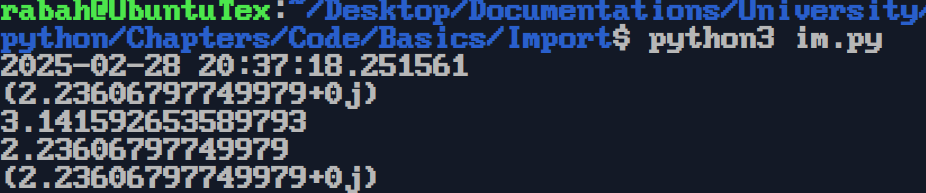
\includegraphics[width = 0.9\textwidth]{Chapters/ScreenShot/Basics/Import/imOutput.png}
\end{center}

\newpage


\section{Operators}
\begin{prettyBox}{Operators}{myblue}
\begin{itemize}
    \item \textbf{Arithmetic Operators}:
        \begin{itemize}
            \item \texttt{+} : Addition
            \item \texttt{-} : Subtraction
            \item \texttt{*} : Multiplication
            \item \texttt{/} :  Float division 
            \item \texttt{//} : Integer division 
            \item \texttt{\%} : Modulo 
            \item \texttt{**} : Exponentiation (power)
            \item \texttt{=} : Assignment 
        \end{itemize}
    
    \item \textbf{Comparison Operators}:
        \begin{itemize}
            \item \texttt{==} : Equal to 
            \item \texttt{!=} : Not equal to 
            \item \texttt{>} : Greater than
            \item \texttt{<} : Less than
            \item \texttt{>=} : Greater than or equal to
            \item \texttt{<=} : Less than or equal to
        \end{itemize}

    \item \textbf{Logical Operators}:
        \begin{itemize}
            \item \texttt{and} : Logical AND 
            \item \texttt{or} : Logical OR 
            \item \texttt{not} : Logical NOT 
        \end{itemize}
\end{itemize}
\end{prettyBox}

\newpage
\section{Control Structures}
\begin{prettyBox}{Control Structures}{myblue}
Python does not use curly braces (\{\}) to define control structures, classes, or functions.  
Instead, it relies on indentation to determine code blocks 4 spaces.In this section, we will explore all control structures with syntax and examples.
\end{prettyBox}

\vspace{1cm}
\subsection{If Statement}
\textbf{\underline{Syntax}}\\[0.1cm]
\lstinputlisting[style=pythonstyle]{Chapters/Code/Basics/Control/synif.py}


\vspace{0.8cm}

\textbf{\underline{Example}}\\[0.1cm]
\lstinputlisting[style=pythonstyle]{Chapters/Code/Basics/Control/if.py}

\vspace{0.35cm}
\begin{center}
    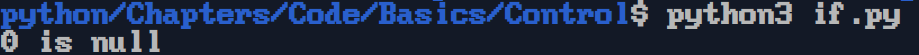
\includegraphics[width = 0.9\textwidth]{Chapters/ScreenShot/Basics/Control/ifOutput.png}
\end{center}

\newpage
\subsection{Match Statement(Switch Case)}
\textbf{\underline{Syntax}}\\[0.1cm]
\lstinputlisting[style=pythonstyle]{Chapters/Code/Basics/Control/synswitch.py}


\vspace{0.8cm}

\textbf{\underline{Example}}\\[0.1cm]
\lstinputlisting[style=pythonstyle]{Chapters/Code/Basics/Control/switch.py}

\vspace{0.35cm}
\begin{center}
    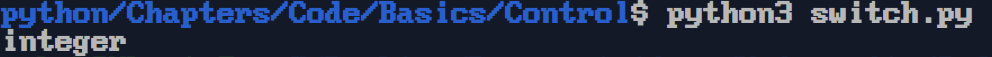
\includegraphics[width = 0.9\textwidth]{Chapters/ScreenShot/Basics/Control/switchOutput.png}
\end{center}

\newpage
\subsection{While Loop}
\textbf{\underline{Syntax}}\\[0.1cm]
\lstinputlisting[style=pythonstyle]{Chapters/Code/Basics/Control/synwhile.py}


\vspace{0.8cm}

\textbf{\underline{Example}}\\[0.1cm]
\lstinputlisting[style=pythonstyle]{Chapters/Code/Basics/Control/while.py}

\vspace{0.35cm}
\begin{center}
    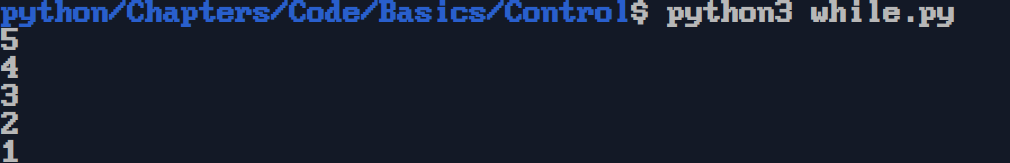
\includegraphics[width = 0.9\textwidth]{Chapters/ScreenShot/Basics/Control/whileOutput.png}
\end{center}

\vspace{1cm}
\subsection{For Loop}
\textbf{\underline{Syntax}}\\[0.1cm]
\lstinputlisting[style=pythonstyle]{Chapters/Code/Basics/Control/synfor.py}


\newpage

\textbf{\underline{Example}}\\[0.1cm]
\lstinputlisting[style=pythonstyle]{Chapters/Code/Basics/Control/for.py}

\vspace{0.35cm}
\begin{center}
    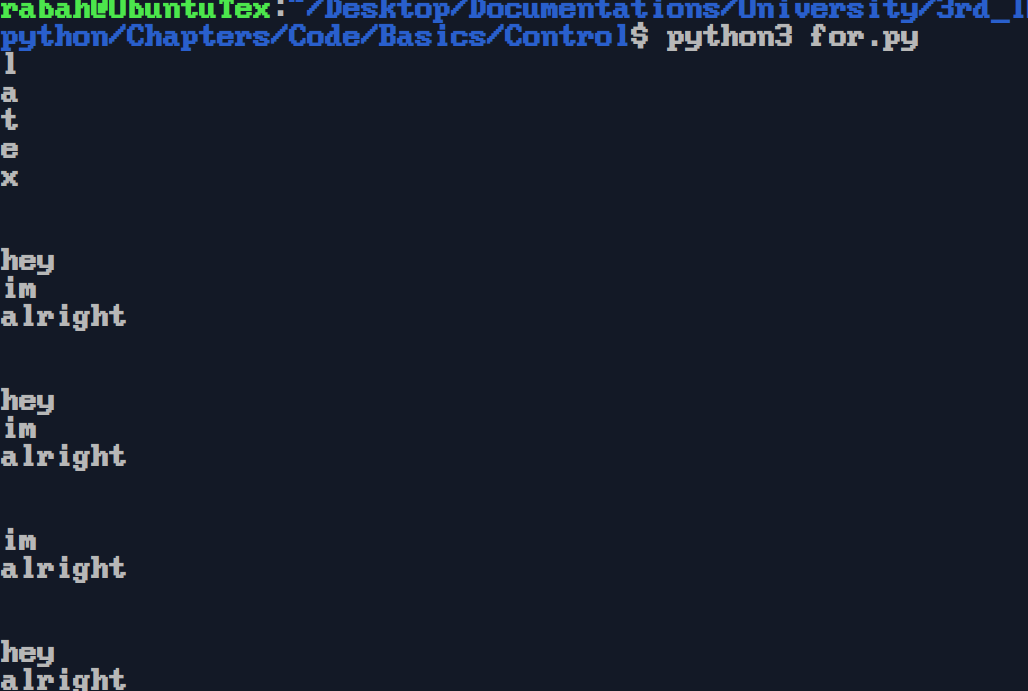
\includegraphics[height = 0.4\textheight]{Chapters/ScreenShot/Basics/Control/forOutput.png}
\end{center}

\newpage
\section{Function}
\textbf{\underline{Syntax}}\\[0.1cm]
\lstinputlisting[style=pythonstyle]{Chapters/Code/Basics/Function/synfunc.py}


\vspace{0.5cm}

\textbf{\underline{Example}}\\[0.1cm]
\lstinputlisting[style=pythonstyle]{Chapters/Code/Basics/Function/func.py}

\vspace{0.35cm}
\begin{center}
    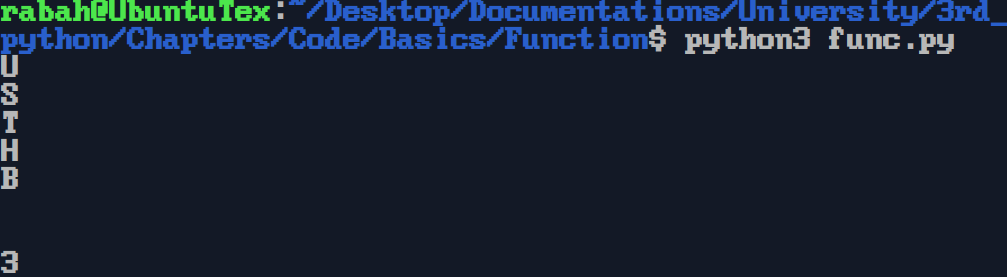
\includegraphics[width = 0.9\textwidth]{Chapters/ScreenShot/Basics/Function/funcOutput.png}
\end{center}

\newpage

\section{NamedTuple}
\begin{prettyBox}{NamedTuple}{myblue}
NamedTuples are similar to structures in C. The key difference is that they have the same properties as tuples, meaning their elements are immutable, so we cannot modify them directly only override them with new ones.\\[0.05cm]
To create a NamedTuples, we need to import the \texttt{namedtuple} function from the \texttt{collections} module. It takes the name of the tuple and its attributes as parameters.
\end{prettyBox}

\vspace{1cm}
\textbf{\underline{Syntax}}\\[0.1cm]
\lstinputlisting[style=pythonstyle]{Chapters/Code/Basics/Struct/synst.py}

\vspace{0.5cm}

\textbf{\underline{Example}}\\[0.1cm]
\lstinputlisting[style=pythonstyle]{Chapters/Code/Basics/Struct/st.py}

\vspace{0.35cm}
\begin{center}
    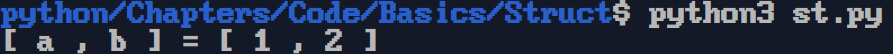
\includegraphics[width = 0.9\textwidth]{Chapters/ScreenShot/Basics/Struct/stOutput.png}
\end{center}


